\documentclass{article}
\usepackage{a4}
\usepackage{epsfig}
\usepackage{url}
\newcommand{\etal}{\emph{et al.}}
\let\shortcite\cite

\bibliographystyle{unsrt}

\title{A Notation Language for Bispecific Antibody Formats (Antibody
Markup Language) and Software for Obtaining Expressions for Desired
Antibodies (abYdraw)}
\author{James Sweet-Jones, Maham Ahmad, Andrew C.R. Martin\\
Institute of Structural and Molecular Biology,\\
Division of Biosciences, University College London,\\
Darwin Building, Gower Street,\\
London, WC1E 6BT, UK}

\begin{document}
\maketitle

\begin{abstract}
Bispecific antibodies (BsAbs) are an up-and-coming class of biologic
drugs that differ from monoclonal antibodies through their ability to
bind to more than one type of antigen. As techniques to generate such
molecules have diversified, so have their formats and need for
standard notation. Previous efforts for developing a notation language
for macromolecule drugs have been insufficient for describing
BsAbs. Here, we present Antibody Markup Language (AbML), a new
notation language specifically for antibody formats which overcomes
the limitations of existing languages and can notate a great diversity
of current BsAb formats. To assist users in this language we also
developed a tool, abYdraw, that may draw antibody schematics from AbML
descriptor strings or generate a descriptor string from a drawn
antibody schematic. AbML has potential to become a standardised
notation for describing new BsAb formats entering clinical trials.
\end{abstract}

\section{Introduction}

Immunoglobulins (IgG), or antibodies, have become useful molecular
tools in biology and medicine due to their natural ability to bind a
specific antigen. When clonally expanded, monoclonal antibodies (mAbs)
have applications spanning molecular diagnostic assays, to medical
imaging and of course, as drug therapeutics \cite{ma:2021}.
Bispecific Antibodies (BsAbs) are specially engineered proteins
that differ from naturally occurring mAbs in their ability to bind to
more than one type of antigen. Depending on the number of different
antigens the molecule in question reacts with, antibodies can be
considered trispecific or tetraspecific, but these will all be called
BsAbs in this report. This makes them a versatile class of molecules
which has become a keen focus of therapeutics in clinical trials
because their bispecificity allows proximally gathering two molecules,
two cells, or one of either to initiate a reaction or neutralise an
infectious agent \cite{fan:2015}. Logically this has given them
great interest in the field of immunomodulatory cancer treatments
\cite{labrijn:2019}, which there are currently two FDA-approved
BsAb drugs: blinatumomab and catumaxomab
\cite{wilke:2017,seimetz:2011} with another, emicizumab, approved for
Factor~VIII deficiency haemophilia \cite{schmitt:2021}. 

The engineering of these molecules has evolved over time since their
inception in the 1970s. At first, the quadroma was to fuse two
hybridoma cell lines, used for generating mAbs which would then result
in some cases where two halves of different Fab fragments form
heterodimers which results in a molecule with two specificities
\cite{milstein:1983,kontermann:2015}. These
techniques offer poor yield due to the disfavoured formation of the
desired heterodimers and so efforts for more scalable synthesis have
led to new techniques of BsAb generation \cite{spiess:2015}. 

DNA recombination has allowed greater flexibility in designing  BsAbs
with IgG-like formats, which can be done by appending additional Fv
fragments at the N- or C- terminus of IgG light or heavy chains
\cite{brinkmann:2017}. This may generate a BsAb fragments 
can dimerise to give a symmetrical molecule which is favoured in the
reaction. Additional residue mutations for knobs-in-holes (KIH)
formats \cite{ridgway:1996} as well as positively and negatively
charged formats \cite{gunasekaran:2010} have assisted in chain
pairing to make the desired antibody format more favourable when
pairing unsymmetrical formats \cite{spiess:2015}.   

Furthermore, recombination also allows linking of VH and VL domains to
give single chained Fv (scFv) fragments or camelid single domain Fv
fragments (nanobodies), which may be sequentially added by engineered
linkers to allow for more specificities along one protein chain
\cite{legall:1999}. Protein engineering allows for generation of 
smaller fragment based BsAbs including 2-chained diabodies or a single
chained sequence of scFvs. These Non-IgG-like molecules are
advantageous because they are easier to produce,  and have lower
immunogenicity risk, but these molecules are limited by short
half-lives, which can be extended through human serum albumin (HSA)
ligation or polyethelene glycol(PEG)-ylation or the addition of
disulphide bonds \cite{kontermann:2011,ma:2021}. 

Most recently chemical conjugation allows modularity of domains which
has given rise to great diversity in structures and presentation of
these molecules \cite{spiess:2015}. In addition to ligating antibody
fragments as seen in the ``Dock and Lock'' format,
antibody-drug-conjugates (ADCs) and fusion proteins have become
popular as methods of delivering small molecule drugs to an intended
target \cite{sau:2017}. Finally, the potential of chemical ligation
has demonstrated production of BsAbs by appending two IgG molecules to
give IgG-IgG molecules \cite{szijj:2021}.  

Improvements in synthesis now leading to be more successful drugs and
because of the increased diversity of BsAbs available, they require
standardised formats for description and annotation when they are
submitted for clinical trials. HELM notation is a useful tool for
noting biologics which tend to be complex, large macromolecules,
including antibodies and an editor was also developed to assist in
generating expressions that display the molecule described
\cite{zhang:2012}. Whilst this is suitable for standard IgG molecules,
it has shortcomings when it is used for BsAbs. The greatest point
which makes HELM unsuitable for BsAbs is that it does not allow for
notation of Fv fragment specificities or to add comments or notes
about the type of extra domains that can be added to an IgG
molecule. Furthermore, the HELM editor does not have specific
expressions for antibody-based drugs as it requires amino acid
sequences to draw a schematic of a molecule, which is not suitable
when describing fragmented BsAbs. Due to the gaining popularity of
BsAbs and the unsuitability of current macromolecule notation, it
presents a case to develop a new notation language that adequately
describes the ever-increasing diversity of BsAbs.

In this paper, we present a new BsAb notation language, Antibody
Markup Language (AbML), which we demonstrate can be used to describe a
variety of current BsAbs formats. Furthermore we apply our language in
a graphical programme, abYdraw, which uses AbML to render schematics
of BsAbs, as well as produces expressions from drawn antibody
schematics.  

\section{Methods}

\subsection{Devising a descriptor language}
We used literature describing the formats of over 60 BsAbs to develop
our description language \cite{spiess:2015}. An effective notation
language must be simply structured but can carry as much information
as needed. Using the documentation of the HELM descriptor language
\cite{zhang:2012}, it was decided that our language would be
structured similarly, but correct for instances where HELM is not
appropriate for BsAbs. We adopt similar domain type characters in AbML
but remove the need to specify a constant heavy (CH) domain and
comment it as to which CH type it is. Similarly we decided to use \verb|"-"|
characters to indicate connections between domains but we also include
hinges and linkers as a type of connector-based domain rather than
having to specify linkers as an extra type of domain. Furthermore,
disulphide bonds between interacting domains were to be shown as these
are important in stabilising chain interactions. Finally it was
decided to incorporate a comment system would to describe
modifications made to the BsAb and denote \verb|"X"| domains which are not in
the standard domain types.  

\subsection{Developing abYdraw}
When it had been shown the descriptor language could be successfully
applied to a variety of  BsAb types, our next step was to make this
language accessible. The most suitable way for that was to design a
programme which would give researchers the expression for their
antibody of interest and allow them to save both the expression and a
rendering of the schematic. abYdraw was written in Python3 and given a
graphical user interface with TKinter, a standard Python package. 


\begin{figure}
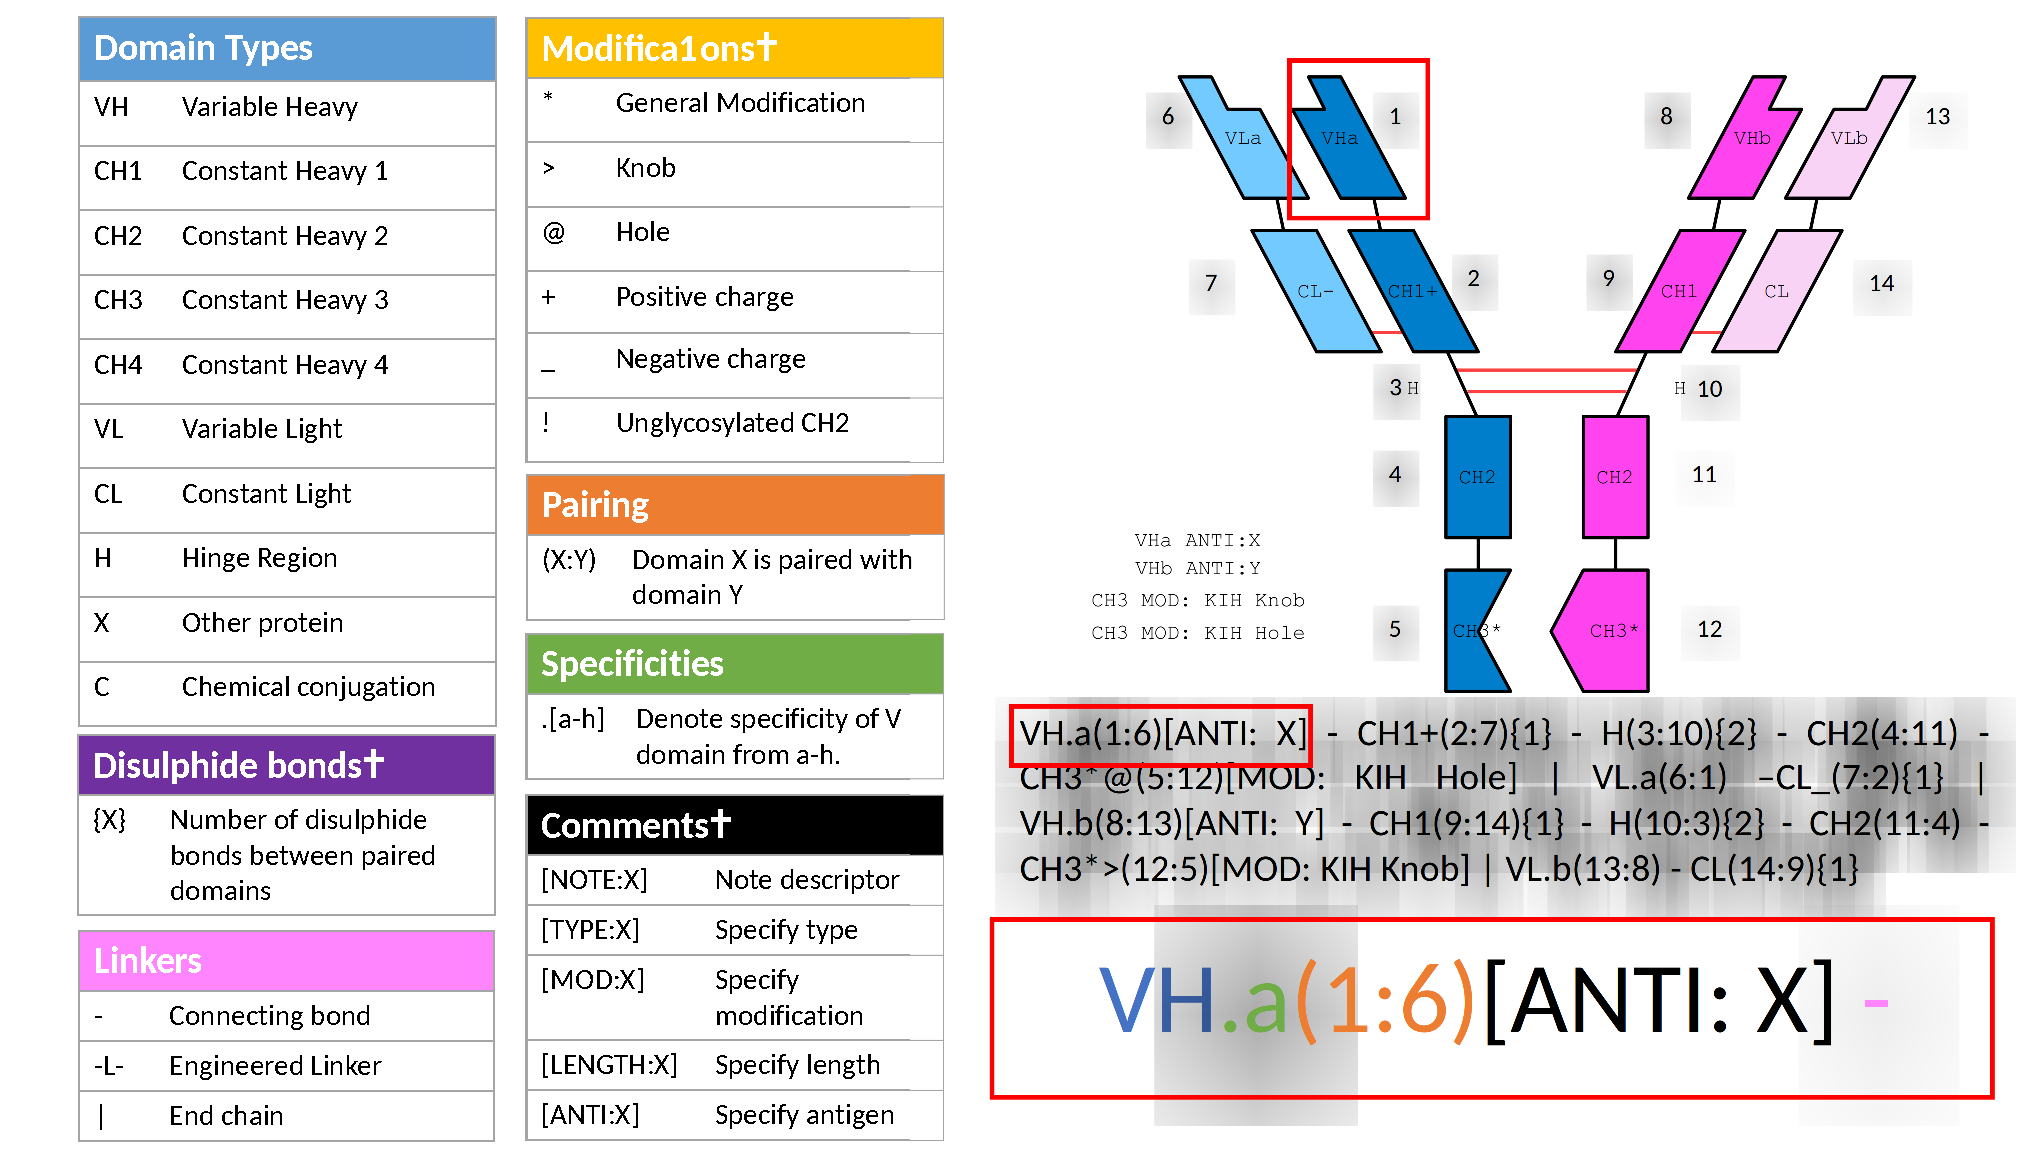
\psfig{width=\columnwidth,file=Figure1.eps}
\caption{\label{fig:1} AbML Guidesheet Explaining the Properties of
the Language. All possible domain types, modifications, linkers and
comment types as well as how to notate pairings and dislphide bonds
are given in colour-coded fashion to the example antibody domain
highlighted in red. Antibody schematic was rendered with abYdraw and
numbers represent the numbering of each domain given in AbML and
labelled on the schematic.}
\end{figure}

\section{Results}

\subsection{Antibody Markup Language}
AbML is based on describing protein domains, arranged in a string and
separated by connecting bonds, which represents a chain from a BsAb
from N-terminus to C-terminus. Each domain is numbered sequentially in
order of its appearance in the expression unless referring to a
previously notated domain. Domains are connected by \verb|"-"| characters
posing as linkers between domains. Chains are separated by \verb."|".
characters and those which are part of the IgG molecule can be
presented in any order but additional fragments that interact with it
typically are noted last. Each chain must have at least one domain
that interacts with another domain on a different chain. Chains that
do not interact with the others are considered different
antibodies. Whitespace, including line breaks are ignored in AbML
except for comments given in square braces. What follows is an
in-depth description of how units link together to generate a complete
expression. 

Domains of the antibody are given in a format that aims to convey as
much information about the domain without becoming overly
complex. Notating domains always begins with the type of domain in
question. Possible domains include [\verb|"VH"|, \verb|"VL"|,
\verb|"CH1"|, \verb|"CH2"|, \verb|"CH3"|, \verb|"CH4"|, \verb|"CL"|,
\verb|"X"|, \verb|"C"|, \verb|"H"|] which are explained in the
language guide sheet (Figure~\ref{fig:1}). Domains containing
\verb|"X"| are considered extra domains that are not part of a
standard immunoglobulin which will usually be explained by comments.

Specific modifications notated by special characters can follow the
domain type which include \verb|"@"| and \verb|">"| for KIH pairing
with holes and knobs given respectively or \verb|"+"| and \verb|"_"|
denoting a positively or negatively charged domain. General
modifications are given with a \verb|"*"| which can be elaborated by a
comment. Modification symbols can appear in any order when they
immediately succeed the domain type in the expression however AbML
does not accommodate combinations where \verb|"@"| appears with
\verb|">"| or \verb|"+"| appears with \verb|"_"| because these are
contradictory adaptations. Similarly, \verb|"!"| can only appear in
domains of type \verb|"CH2"| as it specifies this domain is
unglycosylated.

If applicable, Fv specificities can be notated by \verb|"."| followed by a
letter corresponding to one type of Fv specificity. We provide letters
a-h, with a single letter representing a different antigen specificity
or multiple letters can indicate a combination of
specificities. Typically, an interacting pair of VH and VL domains
should both be assigned identical specificity descriptors but
exceptions apply when two different light chains share a common heavy
chain. 

Following specificities, a bracketed list of the number on that domain
a colon and its interacting domain, although it is optional to exclude
interacting domains e such as the case of nanobodies or to include a
list of interactions when describing an \verb|"X"| domain
multimer. Possible domain pairings include \verb|VH:VL|,
\verb|CH1:CL|, \verb|CH2:CH2|, \verb|CH3:CH3|, \verb|CH4:CH4|,
\verb|H:H|, \verb|X:X|, and \verb|C:C|. Further optional curled braces
notating the number of disulphide bonds between the previously
specified interacting domains.

Each domain may be given an optional comma-separated list of comments
within a set of  squared braces. These comments can denote types of
other protein domains not notated in the language as well as antigen
specificities or the length of a domain or linker. A full list of
keywords and modifications can be found on the AbML descriptor sheet
(Figure~\ref{fig:1}).

Domains are linked by \verb|"-"| which represents an ordinary peptide linker
between bonds, however these can be changed to hinge regions or
artificially engineered linkers (\verb|-L-|) which may carry more information
about pairing. disulphide bond connections noted by sets of round or
curled braces. It is conventional that hinge regions are placed
between CH1 and CH2 domain types and linkers are placed where a
different antibody chain or domain is appended to the IgG molecule,
and between the VH and VL domains of a scFv.  

\subsection{abYdraw}
abYdraw is a graphical programme written in Python3 where users may
input expressions in AbML to obtain a schematic of their designed
antibody by clicking the \verb|"Get Structure"| button. However, the user is
also able to draw antibodies by arranging standard antibody domains
and connecting them with linkers to obtain the appropriate expression
for their design by using the \verb|"Get Sequence"| button. Once the sequence
is obtained for the drawing, using \verb|"Get Structure"| will re-render the
schematic automatically. Both functions can run in sequence using the
\verb|"Tidy"| button. The programme will also print out comments made in the
expression and highlight the domain linked to those comments. abYdraw
can be used to export these schematics as figures for future
publications and generate a standardised expression that may be used
in BsAb annotations.  

The interface draws domains as blocks labelled with their domain type
and modifications given in the expression. Character substitutions
include \verb|"_"| to \verb|"-"| in labels with \verb|"@"| and
\verb|">"| characters also being omitted as these modifications are
used to affect the shape of the domain. Domains are coloured according
to their specificities descriptor. It is possible that chains will
have blocks of different colours when domains of different
specificities are given in the same chain. Variable domains appear
with a cut-out at the top of the domain referring to its
antigen-interacting site which pairs with another to give a complete
Fv fragment. Nanobodies have a unique domain shape reflecting their
single domain Fv fragment as KIH adaptations are displayed by constant
domains with either a cut-out or an extension to their side which
slots together to demonstrate how these domains are paired.

Normal Connections between each domain are given by black lines that
are drawn from the bottom of one domain to the top of the next
domain. Artificial linkers are shown in purple lines, disulphide bonds
are shown by red lines and hinges are shown in dark green. A default
list of colours for all domain and bond types is given in the
programme but these may be changed in settings for the user. Any
comments given in the expression are printed with the domain symbol of
the domain which it applies to the antibody. If multiple comments are
given for a domain, they are printed on the same line. 

Users may draw BsAbs from scratch or begin with a template design of
common BsAb formats that may be manipulated by the user. To Draw
domains, a user must select a specificity and any mods for that domain
and then place it on the canvas. Both specificities and modifications
can be updated whilst on the canvas by selecting a specificity or
modification, but not a domain type. Once drawn, domains may be
translated to a space where they interact with other domains to be
paired. VH and VL domains must face each other to be considered as
interacting. Users can right-click newly drawn domains to change the
direction they are facing. Nanobodies cannot be paired with other
domains as these are single-domain Fv fragments. Bonds connecting
domains must be drawn starting on the previous domain and ending on
the current domain. Disulphide bonds can be drawn starting from either
domain that are supposed to be interacting. To Insert a comment, users
will select which comment type they want, type their comment into the
keypad entrybox and then place the comment inside the domain it is
applicable to.  

\begin{figure}
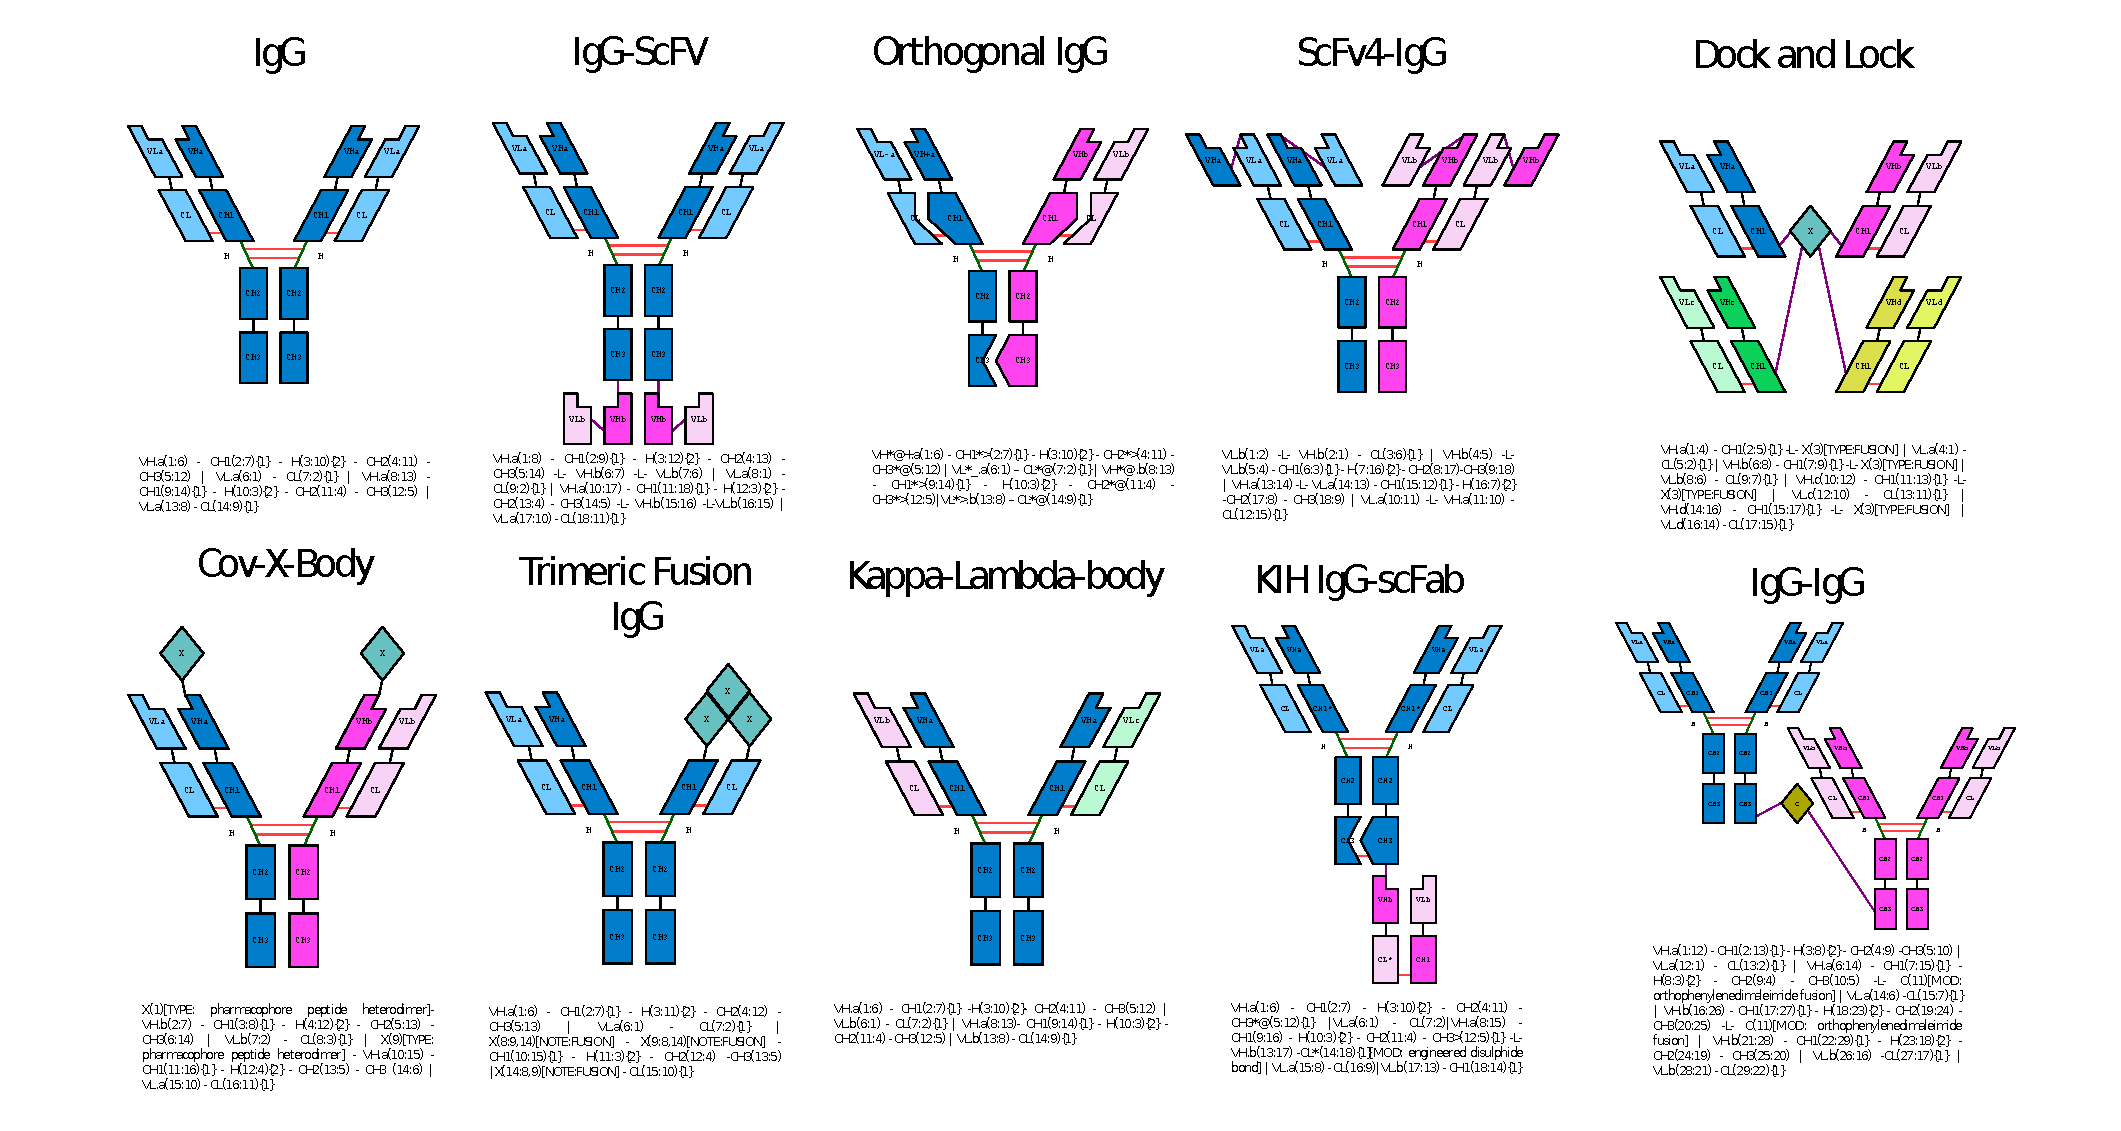
\psfig{width=\columnwidth,file=Figure2.eps}
\caption{\label{fig:2} AbML descriptor strings of commonly-used
4-chain bispecific antibodies. Schematics of antibodies were rendered
in abYdraw.} 
\end{figure}

\begin{figure}
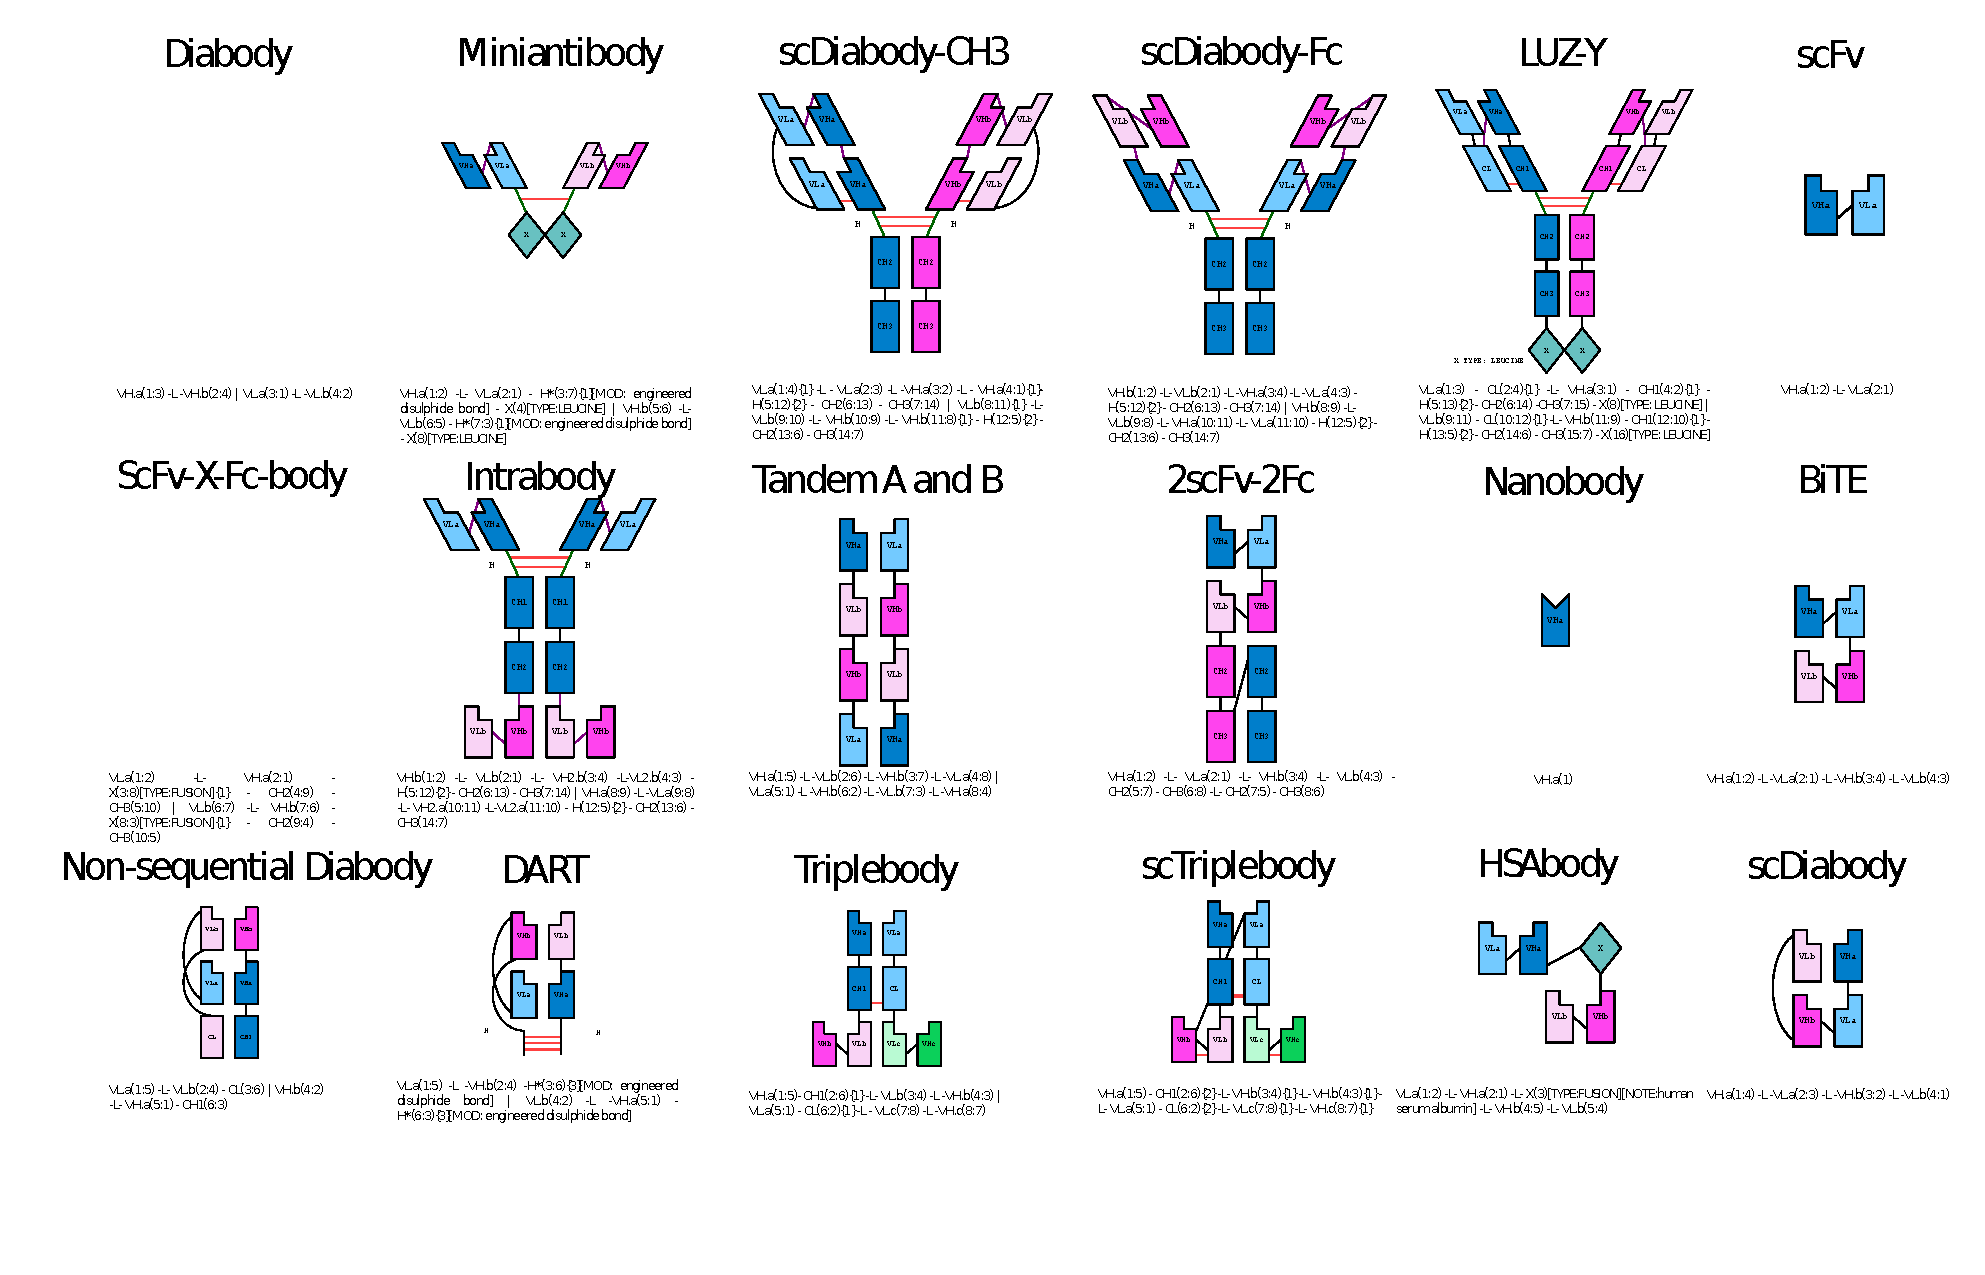
\psfig{width=\columnwidth,file=Figure3.eps}
\caption{\label{fig:3} AbML descriptor strings of commonly-used
2-chain and 1-chain bispecific antibodies. Schematics of antibodies
were rendered in abYdraw.} 
\end{figure}

Figures~\ref{fig:2} and~\ref{fig:3} demonstrate that AbML may be
applied to numerous antibody formats described by Spiess \etal
\shortcite{spiess:2015} and then rendered using abYdraw.


\section{Discussion}

By addressing the pitfalls of currently available notation languages,
we have developed AbML which can be applied to existing BsAbs. Our
language was based on the established HELM notation for macromolecule
biologics but simplified and adapted to specifically describe antibody
formats. The simplicity of AbML over HELM allows greater accessibility
as well as allowing the potential to insert additional modifications
symbols and domain types that will futureproof the language to cope
with the inevitably expanding formats of recombinant and chemically
conjugated BsAbs. This will not always be necessary as \verb|"X"| and \verb|"C"|
domains can be described as a multitude of possible fusion proteins,
drug conjugates and chemical bonds using the comments system, and so
the language should not require constant updating. Despite this
anticipation, it is expected that AbML and abYdraw will require
updating with new formats that emerge. 

We hope that by developing abYdraw, a compiled application which may
generate AbML from an antibody schematic, where the schematic and
expression may be used to describe the BsAb format. Tools such as
abYdraw are intended to make AbML more accessible and promote the use
of AbML to its potential in becoming a widely-used, standardised
notation for describing BsAb formats. To aid this usage, abYdraw
includes a library of commonly used BsAb formats complete with AbML
strings and diagrams that can be used as starting points for
researchers to design new drugs. While the AbYdraw software is
available from GitHub repositories, further developments could be made
to promote it on online by porting it to JavaScript or by installing a
command-line interface that could be installed onto a webpage to make
it more accessible.  


\section{Conclusion}

To Conclude, our annotation language AbML is a new descriptor language
for BsAb formats and has demonstrated its ability application to
existing BsAb formats. We envision this language and its corresponding
tool abYdraw to become useful in the development of future BsAb drugs,
allowing for standardisation of BsAb description as part of ushering
in a new era of BsAb development. Improved descriptions of their
formats will demonstrate the most popular formats and those which are
most likely to work as drugs, therefore prompting greater development
in the bispecific field.  

\section{Software Availability}
Compiled apps for Mac OS and windows are made free to download at:
Source code for this project is also made available at
\url{https://github.com/JamesSweetJones/abYdraw}

\bibliography{abYdraw} 

\end{document}
